\chapter{Introdução}

É  indiscutível que  a web  se tornou  uma tecnologia  essencial  para negócios,
comércio,  educação, engenharia,  entretenimento, finanças,  governo, indústria,
mídia, medicina, política, ciência e  transporte, isso para citar apenas algumas
áreas que têm impacto sobre nossa vida.

\vspace{0.2cm}

No  entanto,  à medida  que  aplicações web  são  integradas  às estratégias  de
negócio, torna-se  cada vez mais  complexo o seu desenvolvimento.   Apesar desse
aumento de responsabilidade, o processo  de engenharia de sistemas web ainda não
é  tão  disciplinado  quanto  à  Engenharia  de  Software  tradicional.   Muitas
aplicações web  continuam a  ser construídas  de uma maneira  {\it ad  hoc}, sem
consideração com os princípios fundamentais da Engenharia de Software.

\vspace{0.2cm}

Dessa  forma, é essencial  que sistemas  passem por  um processo  de engenharia,
denominado Engenharia Web, de forma a construir e implantar uma solução eficaz e
eficiente  e que  atenda às  estratégias de  negócio e  às expectativas  de seus
usuários,  pois como  nos  demais tipos  de  software, é  necessário o  completo
entendimento  do  problema  para  se   projetar  uma  solução  eficaz  que  seja
implementada e testada corretamente.

\vspace{0.2cm}

Nesse contexto, a  Engenharia Web~\cite{Bed12, Pressman09}\index{Engenharia Web}
consiste  em  uma  abordagem  sistemática  e  ágil  para  o  desenvolvimento  de
aplicações  web. A agilidade  implica em  um enfoque  de Engenharia  de Software
enxuto que incorpora ciclos de  desenvolvimento rápidos. E cada ciclo resulta na
implantação de  um incremento da aplicação  web.  Ou seja,  o desenvolvimento da
aplicação web é realizado por meio  da entrega de uma série de versões, chamadas
de  incrementos,  que  fornecem  progressivamente mais  funcionalidade  para  os
clientes à medida que cada incremento é entregue.

\vspace{0.2cm}

Esse material  apresenta o framework web  Grails que é bem  inerente à filosofia
ágil. Na realidade, Grails, por si só não é ágil, pois nenhuma ferramenta por si
só  pode ser  ágil. No  entanto, ele  se encaixa  muito bem  com a  filosofia de
desenvolvimento ágil que sustenta que  a melhor forma de atender às necessidades
dos clientes é por meio da  colaboração de um grupo comprometido de pessoas, que
se concentra na  obtenção de resultados com rapidez, com  o mínimo de sobrecarga
possível~\cite{BA04, Schwaber04}.

\vspace{0.2cm}

O  framework Grails é  inerente a  muitas das  boas práticas  do desenvolvimento
ágil, incluindo as seguintes:

\begin{itemize}

\vspace{0.2cm}
\item  {\bf  Ser  adaptável  à   mudança}:  Graças  ao  seu  mecanismo  de  {\it
  autoreloading}   e  natureza   dinâmica,  Grails   promove  a   mudança   e  o
  desenvolvimento iterativo.

\vspace{0.2cm}
\item  {\bf Entrega  precoce do  software funcional}:  A simplicidade  de Grails
  permite uma  abordagem de desenvolvimento rápido de  aplicações, aumentando as
  probabilidades de  entrega rápida.  Além  disso, Grails prega a  automação dos
  testes   unitários   e    de   integração   (ver   Capítulo~\ref{conclusoes}),
  conscientizando os desenvolvedores de sua importância.

\vspace{0.2cm}
\item {\bf Simplicidade é  essencial}: Grails visa proporcionar simplicidade. Ou
  seja,   Grails   tem   conceitos   complexos   como   ORM   (Object-Relational
  Mapping\footnote{Mapeamento  Objeto-Relacional}),  porém  ela encapsula  esses
  conceitos em  uma API simples.  Mapeamento objeto-relacional é uma  técnica de
  desenvolvimento  de software  que é  utilizada com  o objetivo  de  reduzir os
  problemas inerentes  à utilização conjunta de  banco de dados  relacionais e o
  paradigma de desenvolvimento orientado a objetos. As tabelas do banco de dados
  são  representadas  através de  classes  e os  registros  de  cada tabela  são
  representados como instâncias das classes correspondentes.

\vspace{0.2cm}
\item {\bf Equipe entusiasmada, auto-organizada com o ambiente certo}: Desde que
  Grails  permite aos  desenvolvedores  centrar-se principalmente  na lógica  de
  negócios  necessários para  resolver um  problema  específico --  ao invés  de
  aspectos relacionados  à configuração de sua  aplicação -- a  equipe está mais
  propensa a ter desenvolvedores entusiasmados.

\end{itemize}

\section{Modelo-Visão-Controlador (MVC)}\index{Modelo-Visão-Controlador (MVC)}

\vspace{0.5cm}

Desde que o padrão arquitetural MVC é o alicerce do framework de desenvolvimento
Grails,  torna-se de fundamental  importancia apresentar  um {\it  overview} dos
principais conceitos relacionados a esse padrão arquitetural.

\vspace{0.2cm}

O modelo-visão-controlador  (MVC)~\cite{KP88, Pressman11} desacopla  a interface
com o usuário  da funcionalidade e conteúdo da  aplicação web. Uma representação
esquemática da arquitetura MVC aparece na Figura~\ref{MVCFig}. 

\vspace{0.2cm}

\begin{figure}[htbp]
\centering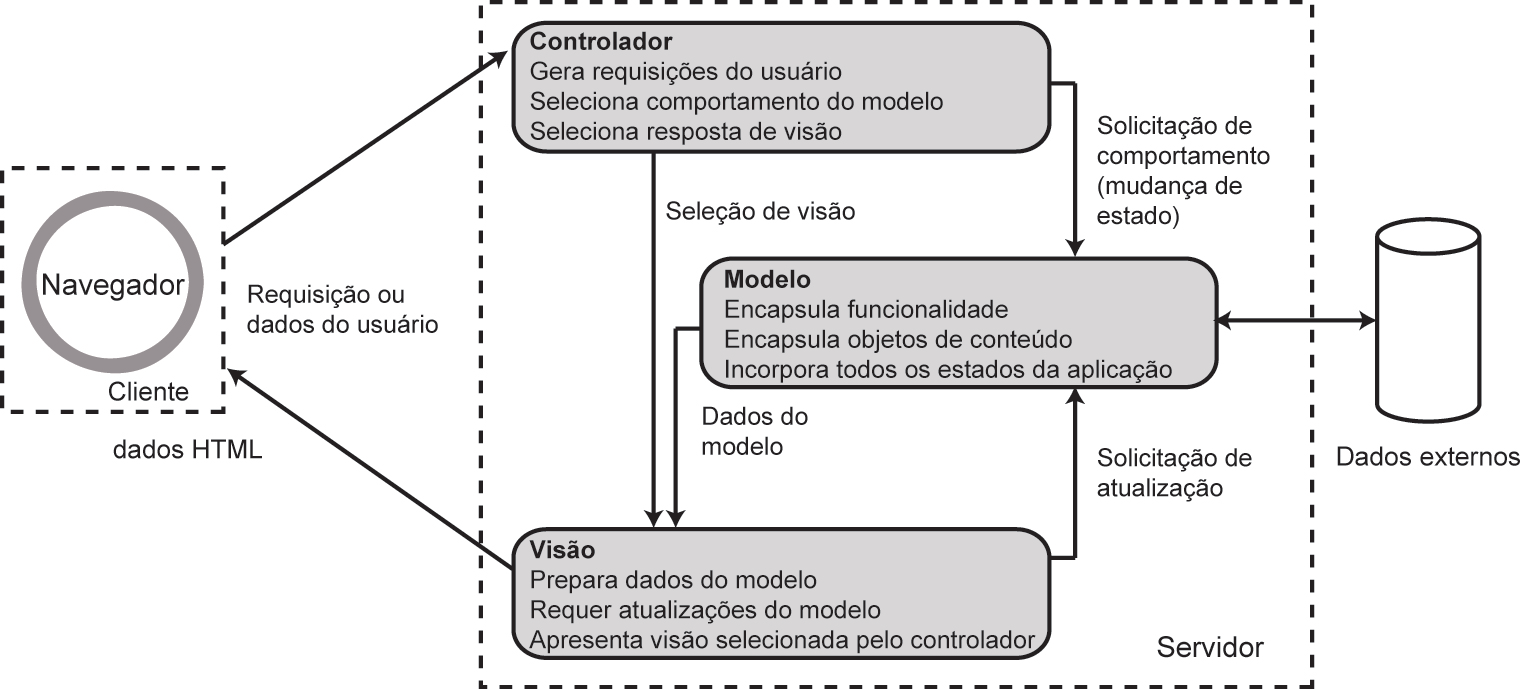
\includegraphics[width=14cm]{MVC}
\caption{Padrão arquitetural MVC}
\label{MVCFig}
\end{figure}

\newpage

Esse padrão  arquitetural define três componentes (Modelo,  Visão e Controlador)
com características bem delineadas:

\begin{itemize}

\vspace{0.3cm}

\item O {\bf Modelo} contém todo  o conteúdo específico da aplicação e lógica de
  processamento, incluindo todos os objetos de conteúdo, acesso a dados externos
  e fontes  de informação, e todas  as funcionalidades de  processamento que são
  específicas da aplicação.  No caso de sistemas que utilizam  bases de dados, o
  modelo mantém  o estado persistente do  negócio e somente ele  pode acessar as
  bases de dados;

\vspace{0.3cm}

\item A {\bf Visão} contém todas as funcionalidades específicas da interface que
  habilita a apresentação de conteúdo e lógica de processamento; e

\vspace{0.3cm}

\item  O {\bf Controlador}  gerencia o  acesso e  a manipulação  do modelo  e da
  visão, bem como coordenar o fluxo de dados entre eles. Em uma aplicação web, o
  controlador monitora a interação com  o usuário e, baseando-se nisso, recupera
  os dados do modelo e utiliza-os para atualizar ou construir a visão.

\end{itemize}

\vspace{0.2cm}

\noindent  Conforme mostra a  Figura~\ref{MVCFig}, as  solicitações ou  dados do
usuário são tratados pelo controlador  que seleciona a visão apropriada com base
na  solicitação do usuário.   Quando o  tipo de  solicitação é  determinado, uma
solicitação  de  comportamento  é   transmitida  ao  modelo,  que  implementa  a
funcionalidade ou recupera  o conteúdo exigido para satisfazer  a solicitação. O
modelo pode  acessar dados  armazenados em um  banco de dados  corporativo, como
parte  de um  armazenamento  de dados  local  ou como  uma  coleção de  arquivos
independentes.   Os  dados  devolvidos   pelo  modelo  devem  ser  formatados  e
organizados pela visão apropriada e depois transmitidos do servidor da aplicação
de    volta   para   exibição    no   navegador    presente   na    máquina   do
cliente~\cite{Pressman11}. 

\section{Grails}

\vspace{0.3cm}

Grails~\cite{Grails}  é   um  framework  web  baseado   no  padrão  arquitetural
MVC~\cite{KP88} que  utiliza a  linguagem Groovy~\cite{Groovy}, executa  sobre a
máquina Virtual Java (JVM) e objetiva a alta produtividade no desenvolvimento de
aplicações      web.      Ele      combina     os      principais     frameworks
({Hibernate\footnote{\url{http://www.hibernate.org/}},
Spring\footnote{\url{http://springsource.org/}}, etc.)  utilizados na plataforma
Java e  respeita o  paradigma {\it Convention-over-configuration}  (Convenção ao
invés de Configuração).

\vspace{0.3cm}

\begin{cBox}
{\bf  Groovy.}   Groovy~\cite{Groovy} é  uma  linguagem  dinâmica,  ágil para  a
plataforma Java inspirada  em Python e Ruby que possui  sua sintaxe semelhante à
de  aplicações  desenvolvidas em  Java.   Apesar de  poder  ser  usada como  uma
linguagem  de  {\it script},  ou  seja, não  gerar  arquivos  executáveis e  não
precisar ser  compilada, Groovy  não se limita  a isso. Aplicações  feitas nesta
linguagem podem  ser compiladas utilizando-se  um compilador Java,  gerando {\it
  bytecodes}  Java (mesmo  formato da  compilação  de uma  aplicação escrita  em
Java),  além disso,  podem ser  utilizadas em  aplicações escritas  puramente em
Java.

A  linguagem foi  desenvolvida em  2004  por James  Strachan.  A  sua sintaxe  é
extremamente  parecida  com a  do  Java,  além  disso, é  possível  ``integrar''
aplicações Java e Groovy de  forma transparente. O Groovy, inclusive, simplifica
a implementação  por ``adicionar'' dinamicamente  às suas classes os  métodos de
acesso ({\bf  get} e {\bf  set}), economizando tempo  e esforço.  O  objetivo de
Groovy é simplificar a sintaxe de Java para representar comportamentos dinâmicos
como consultas  a banco de dados, escritas  e leituras de arquivos  e geração de
objetos em tempo de execução ao invés de compilação~\cite{Groovy}.

\noindent {\it  Convention Over Configuration (CoC)}.  O CoC é  um paradigma que
visa  a diminuir a  quantidade de  decisões que  o desenvolvedor  precisa tomar,
tomando como ``padrão'' algo que é  comumente usado (uma convenção). Se o padrão
escolhido pelo framework for a que o desenvolvedor precisa, este não gasta tempo
tendo que alterá-la. Entretanto, se  ele necessita de algo diferente, fica livre
para configurar  da forma que  desejar. No caso  do Grails, ele  assume diversas
configurações,  tais  como   as  de  banco  de  dados,   as  de  localização  do
código-fonte, entre outras.  \index{Convenção!{\it versus}~Configuração} 
\end{cBox}

\vspace{0.5cm}

Este tutorial apresenta  o framework Grails apoiando o  Desenvolvimento Web Ágil
de  Software.  Uma  aplicação   denominada  {\bf  ControleBancario}  ilustra  as
diferentes etapas do processo de desenvolvimento:

\begin{itemize}

\vspace{0.3cm}

\item O capítulo~\ref{bancario} descreve  a implementação inicial das principais
  funcionalidades dessa aplicação; 

\vspace{0.3cm}

\item O capítulo~\ref{autenticacao} descreve a implementação das funcionalidades
  de autenticação de usuários no contexto dessa aplicação.  

\vspace{0.3cm}

\item  O   capítulo~\ref{autorizacao}  descreve   como  pode  ser   realizada  a
  personalização das funcionalidade presentes na aplicação ao adicionar aspectos
  relacionados à autorização do acesso às funcionalidades. 

%\vspace{0.3cm}

%\item   O  capítulo~\ref{interface}   descreve  como   pode  ser   realizada  a
%personalização  da interface da  aplicação ao  adicionar padrões  de interface.
%Adicionalmente, esse capítulo descreve a  implementação de um serviço {\it web}
%REST e de algumas funcionalidades AJAX na aplicação {\bf ControleBancario}.

\vspace{0.3cm}
  
\item Finalmente, o capítulo~\ref{conclusoes} apresenta o {\it overview} de mais
  algumas  funcionalidades  presentes em  Grails  que  não  foram abordadas  nos
  capítulos anteriores.  
 
\end{itemize}

\subsection{Ambiente de Desenvolvimento}
\index{Ambiente de Desenvolvimento}

\vspace{0.3cm}

Esta  seção   apresenta  alguns  pré-requisitos\footnote{Mais detalhes podem ser
  encontrados em:  \url{http://www.itexto.net/devkico/?p=40}.}  do ambiente para
apoiar o  desenvolvimento. O atendimento desses  pré-requisitos são fundamentais
para a  instalação e configuração do  ambiente de desenvolvimento  que apoiará a
compilação e execução  dos exemplos discutidos neste tutorial.   A instalação do
ambiente é simples e consiste de: 

\hspace{1cm}\\
\noindent{\bf Instalação  da linguagem  Java.}  O Java  Development Kit  (JDK) –
versão  igual ou  superior a  1.5 –  será necessário  para executar  os exemplos
apresentados  nesse  material.   A última  versão  do  JDK  pode ser  obtida  em
{\footnotesize\url{http://java.com/pt_BR/download/index.jsp}}   (Esse   material
utiliza o JDK versão 1.8.0\_77). 

\vspace{0.5cm}

Dicas importantes: (1)  A variável de ambiente {\bf  JAVA\_HOME} precisa apontar
para o diretório onde o JDK foi  instalado. (2) Digite {\bf java -version} em um
terminal    para   verificar    se   o    Java   foi    instalado   corretamente
(Figura~\ref{jdkFig}).

\vspace{0.5cm}

\begin{figure}[htbp]
\centering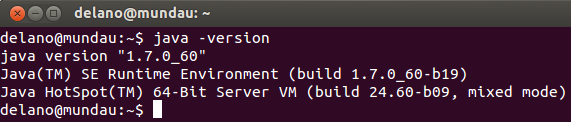
\includegraphics[width=14cm]{java}
\caption{Verificação da instalação do Java}
\label{jdkFig}
\end{figure}

\newpage

\noindent {\bf Instalação  do Grails.}  Nesse tutorial adotou-se  a versão 3.1.4
do         Grails         que         pode         ser         obtida         em
{\footnotesize\url{https://github.com/grails/grails-core/releases/download/v3.1.4/grails-3.1.4.zip}}.  
  
\hspace{1cm}\\
\noindent Após realizar o {\it download}, execute os seguintes passos:

\vspace{0.3cm}

\begin{enumerate}

  \item Descompacte  o Grails em  um diretório e  crie uma variável  de ambiente
    {\bf  GRAILS\_HOME} e  faça-o apontar  para o  diretório onde  o  Grails foi
    descompactado; e

\vspace{0.3cm}
  
  \item Adicione {\bf GRAILS\_HOME/bin} na variável de ambiente {\bf PATH}.

\end{enumerate}

\vspace{0.3cm}

Dica importante: Digite {\bf grails -version} em um terminal para verificar se o
Grails  foi  instalado  corretamente  e  está pronto  para  uso.   Para  maiores
informações sobre a instalação do Grails, consulte o endereço: 
{\footnotesize\url{http://grails.org/Installation+Portuguese}}.  

\vspace{0.5cm}

\noindent {\bf Instalação  de IDE.} O IDE Intellij  é utilizado para desenvolver
as aplicações apresentadas nesse tutorial.   Nesse tutorial foi adotada a versão
2016.1.1  do      IDE Intellij      que      pode      ser      obtida      em
{\footnotesize\url{https://www.jetbrains.com/idea}}

\vspace{0.5cm}

Embora  um  IDE\footnote{Em inglês:  {\it  Integrated Development  Environment}}
facilite  o  desenvolvimento,  o  Grails  não  exige  a  utilização  de  um  IDE
específico.  Todos  os comandos necessários ao desenvolvimento  podem ser feitos
em  um terminal  de comando.   No entanto,  assim como  em outras  linguagens de
programação,  o  IDE  torna  ágil  o processo  de  desenvolvimento  ao  integrar
diferentes funcionalidades  (edição, compilação,  execução, etc.)  e  abstrair a
sintaxe dos comandos necessários  relacionados a essas atividades.  Dessa forma,
fica a critério  do leitor a escolha do IDE mais  adequado às suas necessidades.
Uma lista de IDEs que dão  apoio ao desenvolvimento de aplicações em Grails pode
ser             encontrada             no             seguinte             link:
{\footnotesize\url{https://grails.org/wiki/IDE%20Integration}}. 

\vspace{1cm}

\noindent{\bf Banco de Dados.}\index{Banco~de~Dados}  A instalação do Grails, na
versão        adotada,       já        incorpora       uma        cópia       do
H2\footnote{\url{http://www.h2database.com/html/main.html}},   um   sistema   de
gerenciamento de banco  de dados relacional totalmente implementado  em Java que
disponibiliza um console na URI \url{/dbconsole} (Figura~\ref{H2DBFig}).  

\vspace{0.5cm}

O  SGBD H2  é útil  para aplicações  de demonstração,  mas em  algum  momento os
desenvolvedores    precisarão   de    um   SGBD    mais   robusto    tais   como
MySQL\footnote{\url{https://www.mysql.com/}},
PostgreSQL\footnote{\url{http://www.postgresql.org/}}                           e
Oracle\footnote{\url{http://www.oracle.com/br/database/overview/index.html}}. Desde
que  o GORM ({\it  Grails Object-Relational  Mapping})\index{GORM} é  uma camada
sobre o framework {\it hibernate}, qualquer  banco de dados que possua um driver
JDBC e um dialeto {\it hibernate} pode ser utilizado.

\newpage

\hspace{1cm}\\
\begin{figure}[htbp]
\centering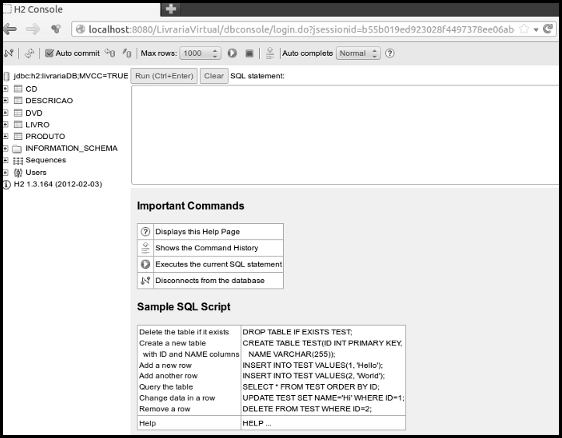
\includegraphics[height=10cm]{H2}
\caption{Console do SGBD H2}
\label{H2DBFig}
\end{figure}

\noindent{\bf  Mecanismo de  {\em build}.}   Desde sua  primeira  versão, Grails
sempre    usou    como    mecanismo     de    {\em    build},    a    ferramenta
Gant\footnote{\url{https://github.com/Gant/Gant}}, que é uma ferramenta bastante
poderosa. No entanto, conforme o tempo foi passando novas opções foram surgindo,
e  desde  a  versão  3,  Grails   adota,  como  ferramenta  de  {\em  build},  o
Gradle\footnote{\url{http://gradle.org/}} que vai além  do Gant: trata-se de uma
ferramenta  de gerencia de  projetos que  lida desde  a gestão  de dependências,
padronização de diretórios, ciclo de vida, construção e muito mais.

\section{Considerações finais}

\vspace{0.3cm}

Esse  capítulo apresentou  um {\it  overview} das  funcionalidades  presentes em
Grails.  Dando continuidade  ao desenvolvimento  em Grails,  o  próximo capítulo
apresenta a  implementação inicial  das principais funcionalidades  da aplicação
{\bf ControleBancario}. 



